% $Id: board1.tex 9375 2021-08-31 13:01:06Z mskala $

%
% MSK 007 Board 1 build instructions
% Copyright (C) 2017, 2020, 2021  Matthew Skala
%
% This program is free software: you can redistribute it and/or modify
% it under the terms of the GNU General Public License as published by
% the Free Software Foundation, version 3.
%
% This program is distributed in the hope that it will be useful,
% but WITHOUT ANY WARRANTY; without even the implied warranty of
% MERCHANTABILITY or FITNESS FOR A PARTICULAR PURPOSE.  See the
% GNU General Public License for more details.
%
% You should have received a copy of the GNU General Public License
% along with this program.  If not, see <http://www.gnu.org/licenses/>.
%
% Matthew Skala
% https://northcoastsynthesis.com/
% mskala@northcoastsynthesis.com
%

\chapter{Building Board 1}

Board~1 has components on both sides, which makes the order of assembly
important; installing the wrong components first may make it difficult to
safely maneuver the soldering iron to install later components without
damaging the already-installed components.  This chapter also includes
instructions on installing the connector on Board~2 that links it to
Board~1.

\section{Preliminaries}

Count out the right number of everything according to the bill of materials. 
There is an abbreviated BOM for Board~1, and the final assembly steps, in
Table~\ref{tab:b1bom}.  In addition to these things you will need your
assembled Boards~2 and~3 from the previous chapters, and the hardware
associated with them.

\noindent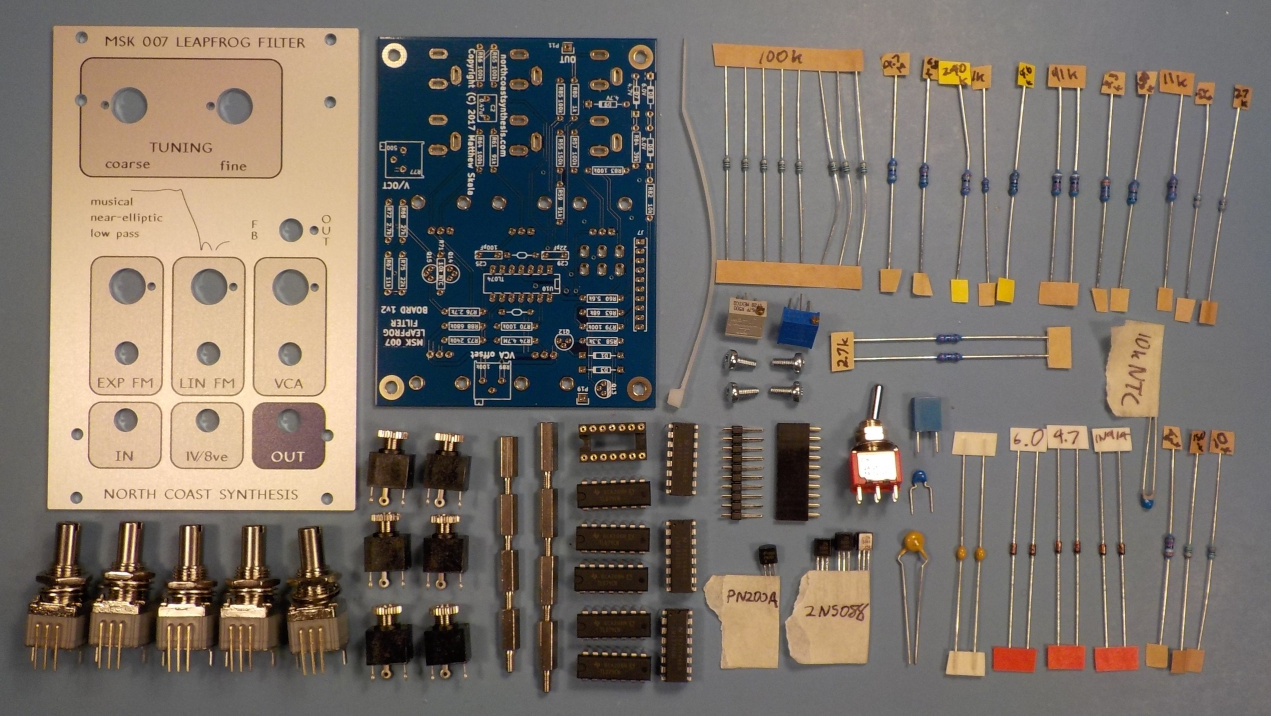
\includegraphics[width=\linewidth]{board1-parts.jpg}

There are two multiturn trimmers to be installed on this board.  Before
installing them, use an ohmmeter to adjust each one to 50\% of its range. 
Measure the resistance along the track, then measure the resistance from the
wiper to one end and adjust to make the wiper half the total track
resistance.  This need not be exact, but it will help with adjustment later,
by reducing issues with interaction among the different settings.  With all
trimmers pre-set to 50\%, the module should basically work even if it is not
at its best, whereas if many are installed at extreme values instead, then
you may have trouble getting it up and running enough to adjust it more
accurately.

\begin{table*}
{\centering
\fbox{This table is not a substitute for the text instructions.}
\vspace{\baselineskip}

\begin{tabular}{rp{1in}cp{3in}}
  \textbf{Qty} & \textbf{Ref} & \textbf{Value/Part No.} & \\ \hline
\input{bomdata-1.tex}
\end{tabular}\par}
\caption{Bill of Materials for Board~1.  Also needed:  knobs, a cable tie,
and module-to-rack mounting~hardware.}\label{tab:b1bom}
\end{table*}

\section{Some notes on knobs}

The first batch of knobs I ordered for North Coast products turned out to
have serious quality problems, specifically with the setscrews that hold the
knobs onto the potentiometer shafts.  Some of the screws had marginal
threads that would strip when the screw was tightened, and I ended up having
to do a bunch of extra testing and ship extra knobs to some customers to
replace any that might fail.  Later batches have also had issues, although
they're under better control now because the bad first batch served as a
warning to step up the testing procedures.  Starting with kits prepared in
August 2019, I switched to blue knobs with 100\%\ testing; in September
2020, I switched to a new manufacturer, and knobs that are a slightly darker
shade of blue.  Although all the knobs I ship in kits now have been tested
and passed at least twice, and should be fine to use, I am also shipping
spare setscrews in any kits with knobs from batches where a signficant
number of knobs failed testing.

Here are some things to be aware of as a kit builder.

\begin{itemize}
\item Some photos in these instructions were taken with the older grey
knobs, and some dealers may still have kits containing grey knobs in their
stock, but newer kits will have blue knobs.

\item Do not overtighten the setscrews when attaching the knobs!  The screw
should be tight enough to hold the knob onto the shaft, but there's no
advantage to making it tighter than that, and overtightening may risk
destroying the screw thread or damaging the drive slot.

\item If, despite my efforts to make sure no bad screws get sent to
customers, you still get a bad screw that cannot be tightened and no spare
for it, then please contact me.

\item If you want to source an exact replacement for the setscrew, it should
be an M3$\times$3mm flat-tip slotted setscrew, which is also sometimes
called a ``grub screw,'' made of RoHS-compliant brass (possibly by
exemption).  Stainless steel is fine too, and I may sometimes ship stainless
steel screws instead of brass if I can find a reliable source for them;
plain steel should not be used here for galvanic corrosion reasons. 
Hex-socket screws are fine if you have the driver for them, but I don't ship
those because I'm not sure all DIY builders do have the right driver.

\item Because it's a standard M3 thread, in a pinch it's possible to
substitute a plain M3 machine screw such as are commonly used with Eurorack
cases, although one of those would obviously look less nice.
\end{itemize}

\section{Fixed resistors}

Resistors are never polarized.  I like to install mine in a consistent
direction for cosmetic reasons, but this is electrically unnecessary.  In
this module, metal film 1\%\ resistors are recommended for all fixed-value
resistors.  These will usually have blue bodies and four colour bands
designating the value, plus a fifth band for the tolerance, brown in the
case of 1\%.  These are the resistors normally shipped in the
North Coast kits, but we may occasionally ship better-tolerance resistors (such
as 0.5\%) if we are able to source them at a good price. 
Accordingly, I mention only the four value band colours for this type of
resistor; if you are using resistors with other codes, you are responsible
for knowing them.  Note that colour codes on metal film 1\% resistors are
often ambiguous (reading from one end or the other end may give two
different values, both plausible) and some of the colours are hard to
distinguish anyway.  If in doubt, always measure with an ohmmeter before
soldering the resistor in place.

\pagebreak

Install the 1k$\Omega$ (brown-black-black-brown) resistor R80.  This
resistor limits the current that can flow on the module output, as well as
separating the output driver op amp and its stability capacitor from any
destabilizing capacitance that may be attached to the output (for instance,
from a long patch cable).  Do not confuse it with the other power-of-ten
resistor values (10k$\Omega$, 100k$\Omega$, and 1M$\Omega$).

\nopagebreak
\noindent\includegraphics[width=\linewidth]{{res-1.0k1}.jpg}

Install the two 2.7k$\Omega$ (red-violet-black-brown) resistors R72 and R76.
These resistors are used in the exponential converter, R72 as part of the
network that scales the control voltage and R76 to control voltage and
current at the output of the servo op amp.  Do not confuse them with the
27k$\Omega$ resistor, which has a similar colour code and is to be
mounted in a PCB footprint near that of R72.

\nopagebreak
\noindent\includegraphics[width=\linewidth]{{res-2.7k1}.jpg}

\pagebreak

Install the 3.3k$\Omega$ (orange-orange-black-brown) resistor R58.
This resistor is used in the linear voltage-to-current converter that
provides control current to the VCA section.

\nopagebreak
\noindent\includegraphics[width=\linewidth]{{res-3.3k1}.jpg}

Install the 5.6k$\Omega$ (green-blue-black-brown) resistor R60.
This resistor converts the exponential converter's output current back to a
voltage for broadcast to the five integrators.

\nopagebreak
\noindent\includegraphics[width=\linewidth]{{res-5.6k1}.jpg}

\pagebreak

Install the 10k$\Omega$ (brown-black-black-red) resistor R82.
This resistor sets the maximum attenuation of the VCA soft-clipping section. 
Do not confuse it with the other power-of-ten resistor values, nor the
11k$\Omega$ resistor.

\nopagebreak
\noindent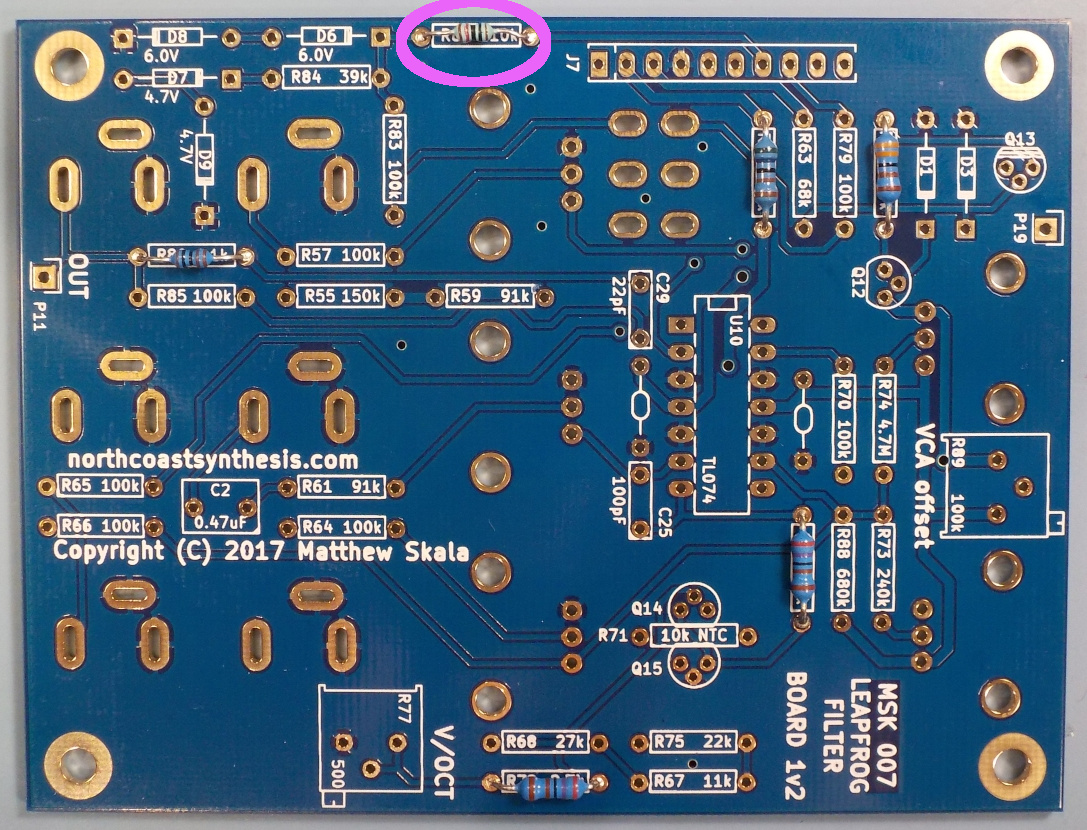
\includegraphics[width=\linewidth]{res-10k1.jpg}

Install the 11k$\Omega$ (brown-brown-black-red) resistor R67.
This resistor is part of the pitch control voltage scaling network.

\nopagebreak
\noindent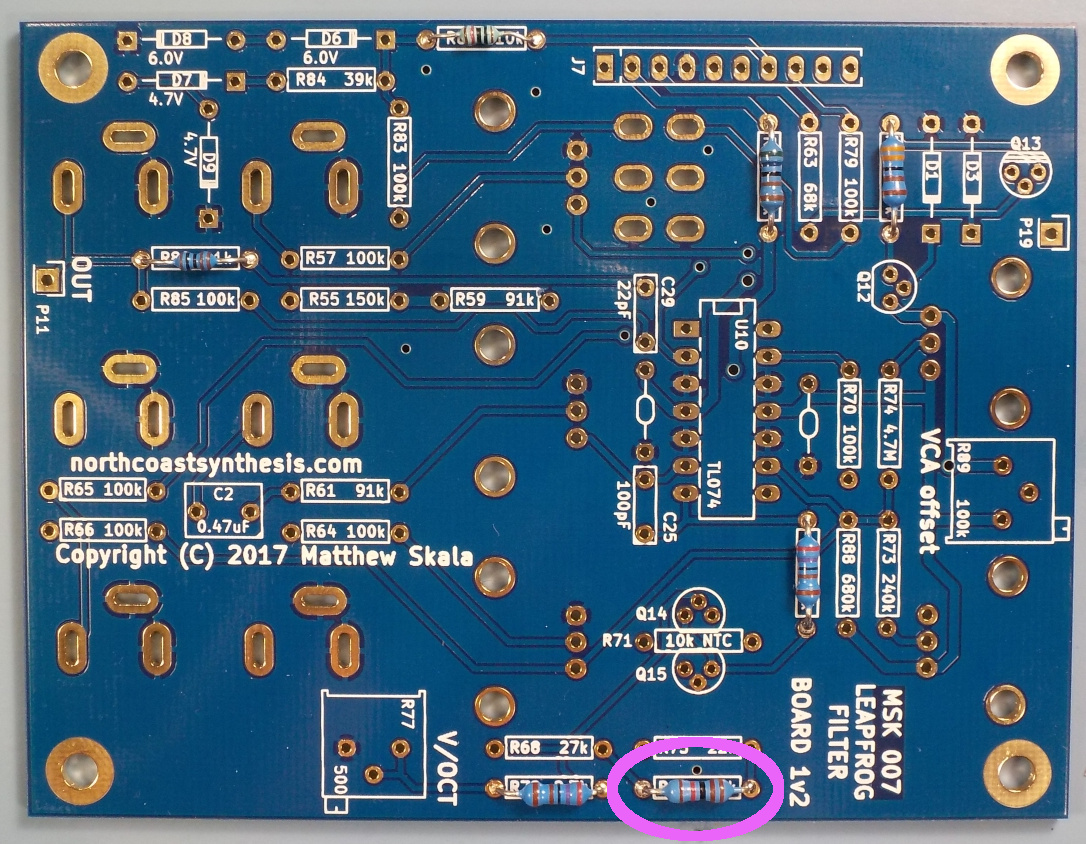
\includegraphics[width=\linewidth]{res-11k1.jpg}

\pagebreak

Install the 22k$\Omega$ (red-red-black-red) resistor R75.
This resistor sets the gain of the op amp in the control voltage scaling
network.

\nopagebreak
\noindent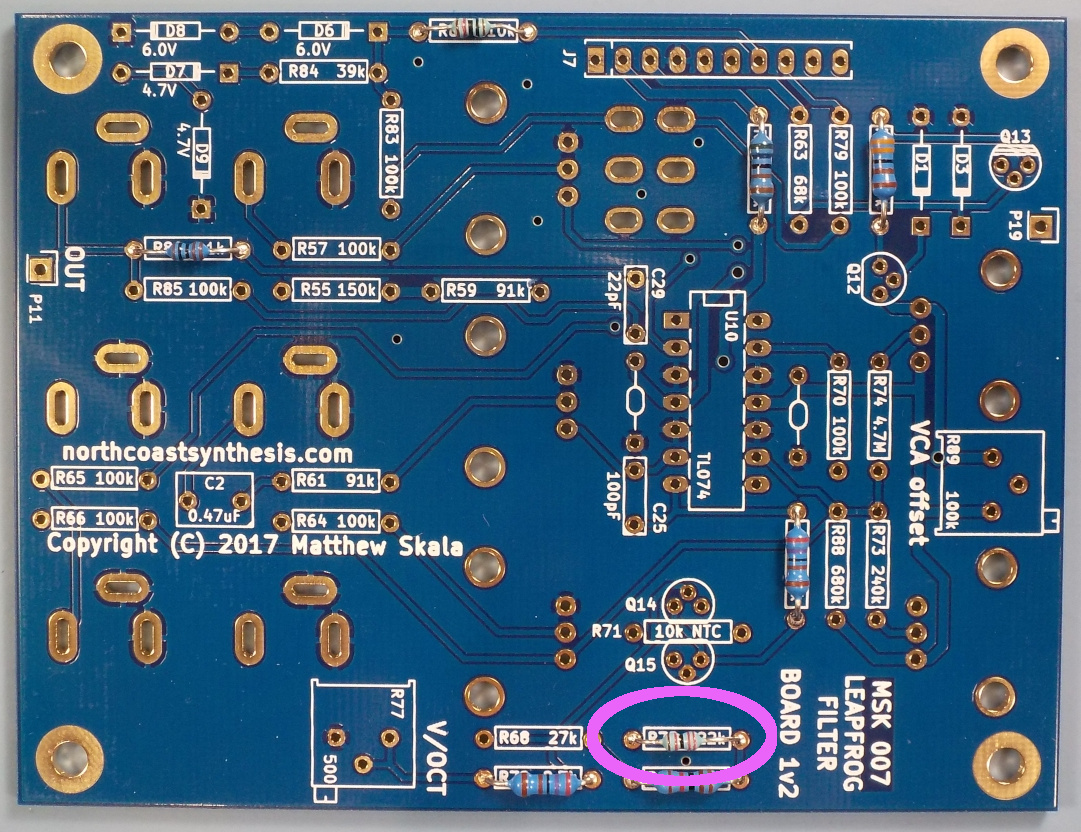
\includegraphics[width=\linewidth]{res-22k1.jpg}

Install the 27k$\Omega$ (red-violet-black-red) resistor R68.
This resistor is another part of the control voltage scaling network.

\nopagebreak
\noindent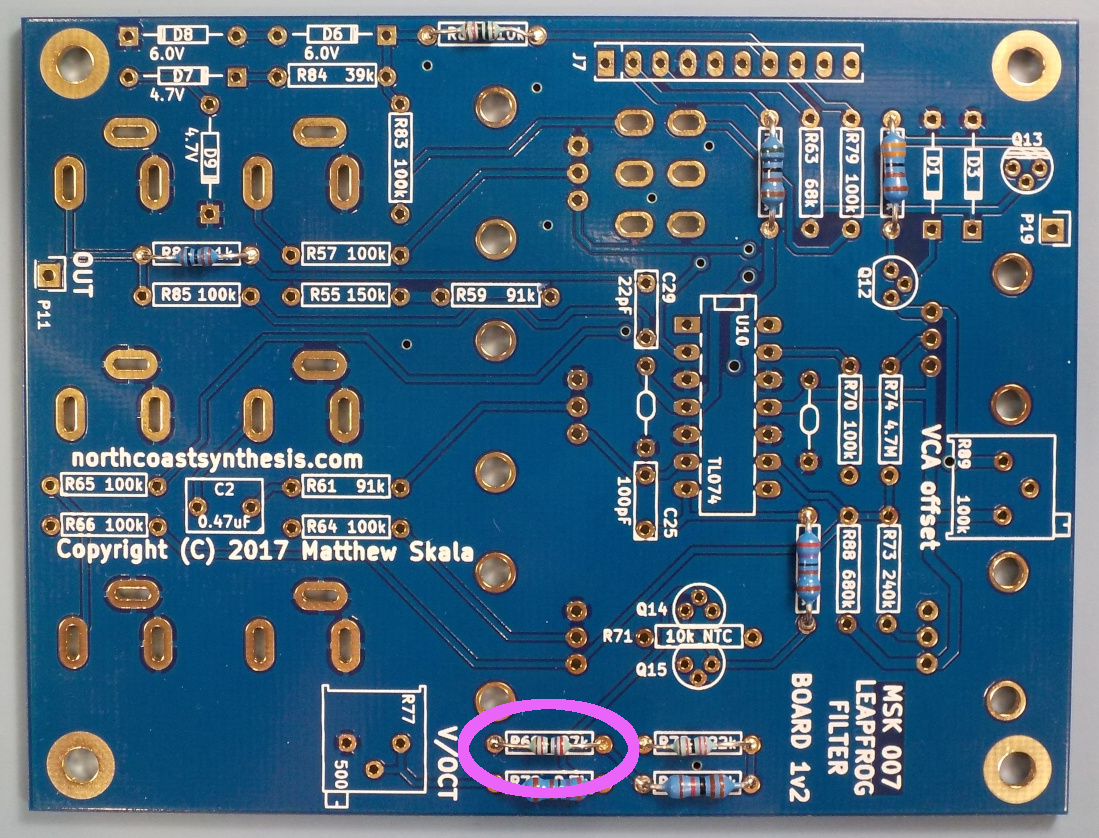
\includegraphics[width=\linewidth]{res-27k1.jpg}

\pagebreak

Install the 39k$\Omega$ (orange-white-black-red) resistor R84.
This resistor sets the mid-level attenuation of the VCA soft-clipping
circuit.

\nopagebreak
\noindent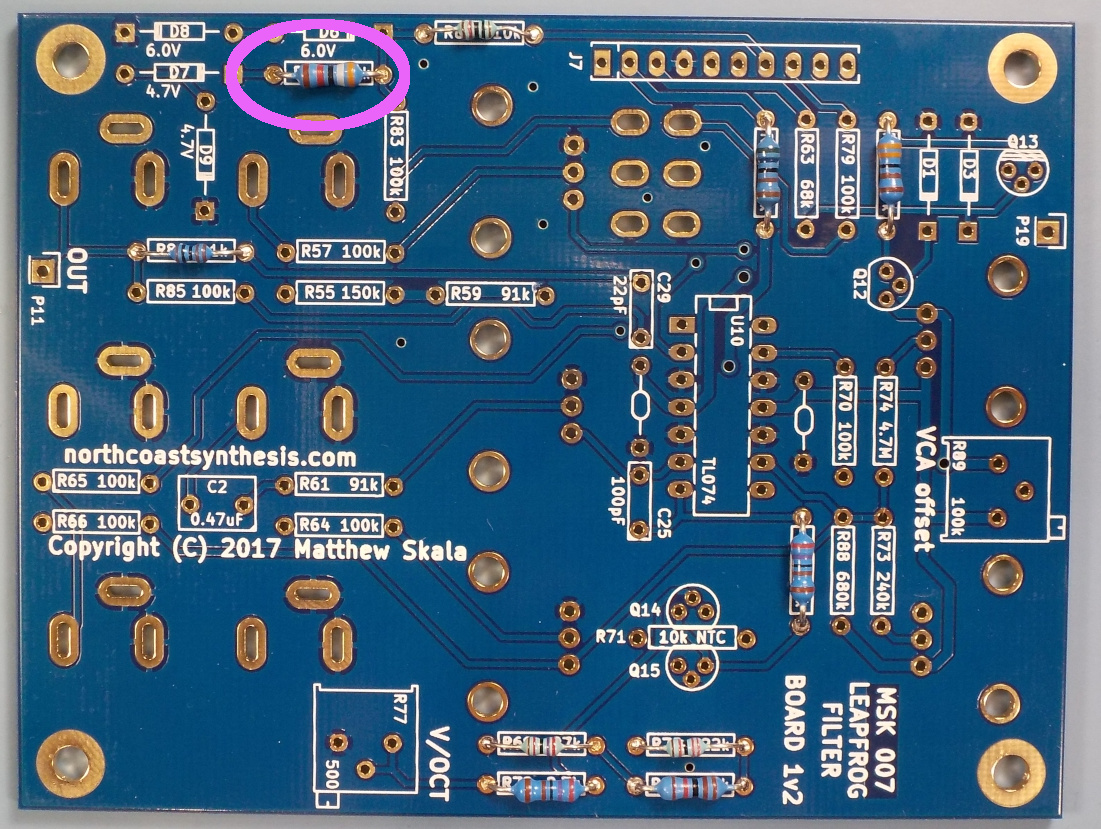
\includegraphics[width=\linewidth]{res-39k1.jpg}

Install the 68k$\Omega$ (blue-grey-black-red) resistor R63.
This resistor pulls down the base of the transistor Q13 to bring the VCA's
zero-gain point near 0V.  Do not confuse it with the 680k$\Omega$ resistor,
which has a similar colour code.

\nopagebreak
\noindent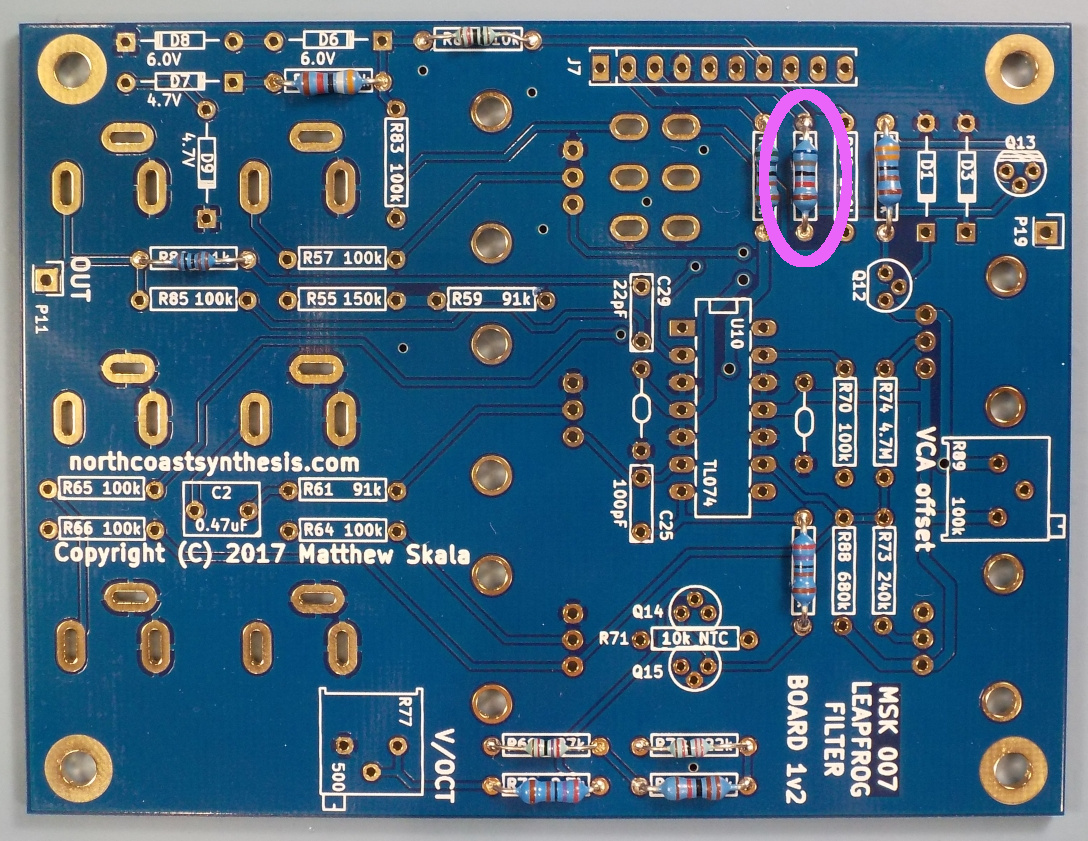
\includegraphics[width=\linewidth]{res-68k1.jpg}

\pagebreak

Install the two 91k$\Omega$ (white-brown-black-red) resistors R59 and R61. 
These two resistors set the reference current for the exponential converter,
and the maximum sensitivity of the linear FM input, respectively.

\nopagebreak
\noindent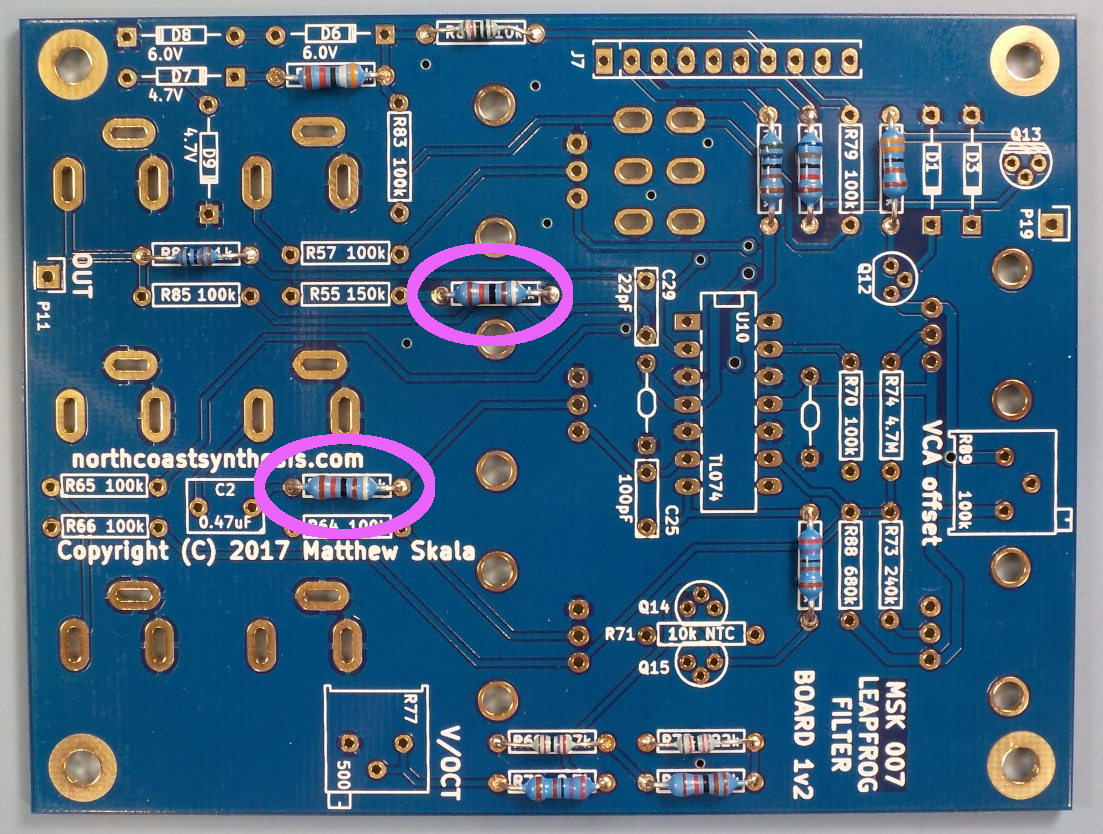
\includegraphics[width=\linewidth]{res-91k1.jpg}

Install the eight 100k$\Omega$ (brown-black-black-orange) resistors R57, R64
through R66, R70, R79, R83, and R85.
These resistors are used in multiple places throughout the input and output
circuits to either set input impedances to Eurorack standard, or set op amp
gain to negative unity by balancing against an input resistor.

\nopagebreak
\noindent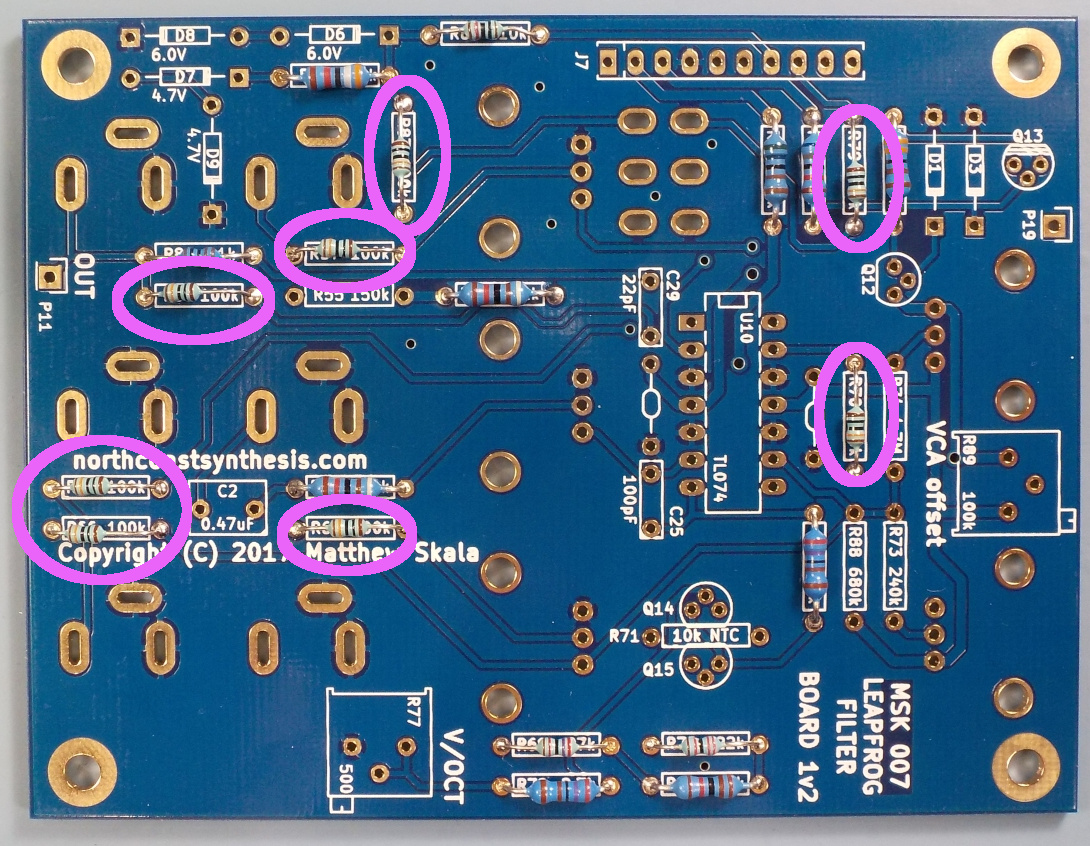
\includegraphics[width=\linewidth]{res-100k1.jpg}

\pagebreak

Install the 150k$\Omega$ (brown-green-black-orange) resistor R55.
This resistor sets the DC normalization for the VCA control input.

\nopagebreak
\noindent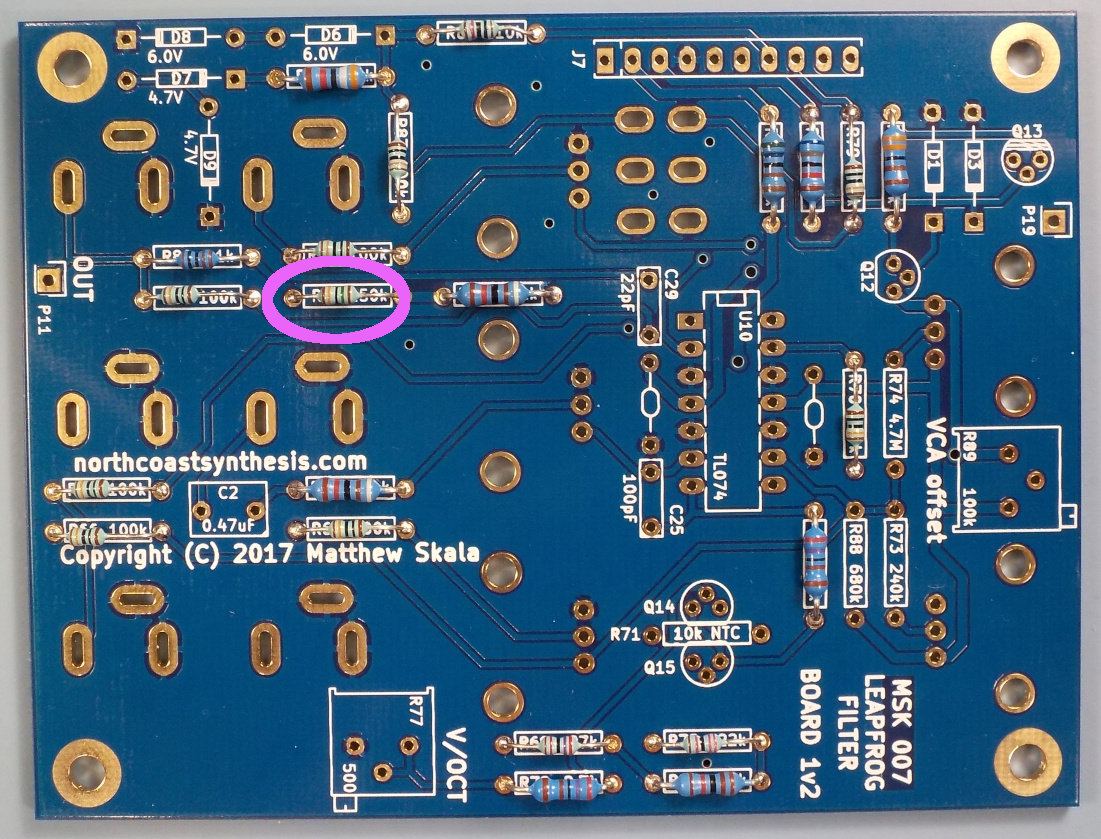
\includegraphics[width=\linewidth]{res-150k1.jpg}

Install the 240k$\Omega$ (red-yellow-black-orange) resistor R73.
This resistor sets the range of the coarse tuning knob to about ten
octaves.

\nopagebreak
\noindent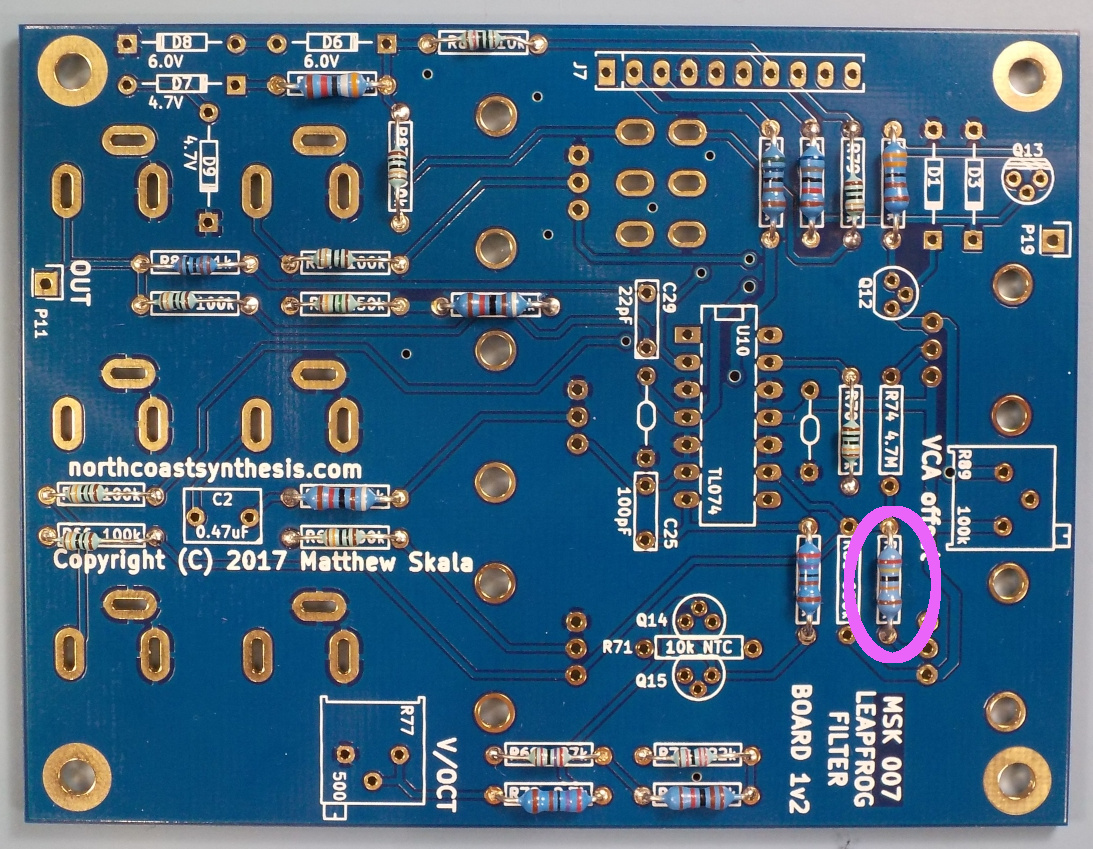
\includegraphics[width=\linewidth]{res-240k1.jpg}

\pagebreak

Install the 680k$\Omega$ (blue-grey-black-orange) resistor R88.
This resistor sets the overall offset of the tuning knobs, for a
non-guaranteed design target of approximately 10Hz to 10kHz cutoff frequency
with zero pitch control voltage.

\nopagebreak
\noindent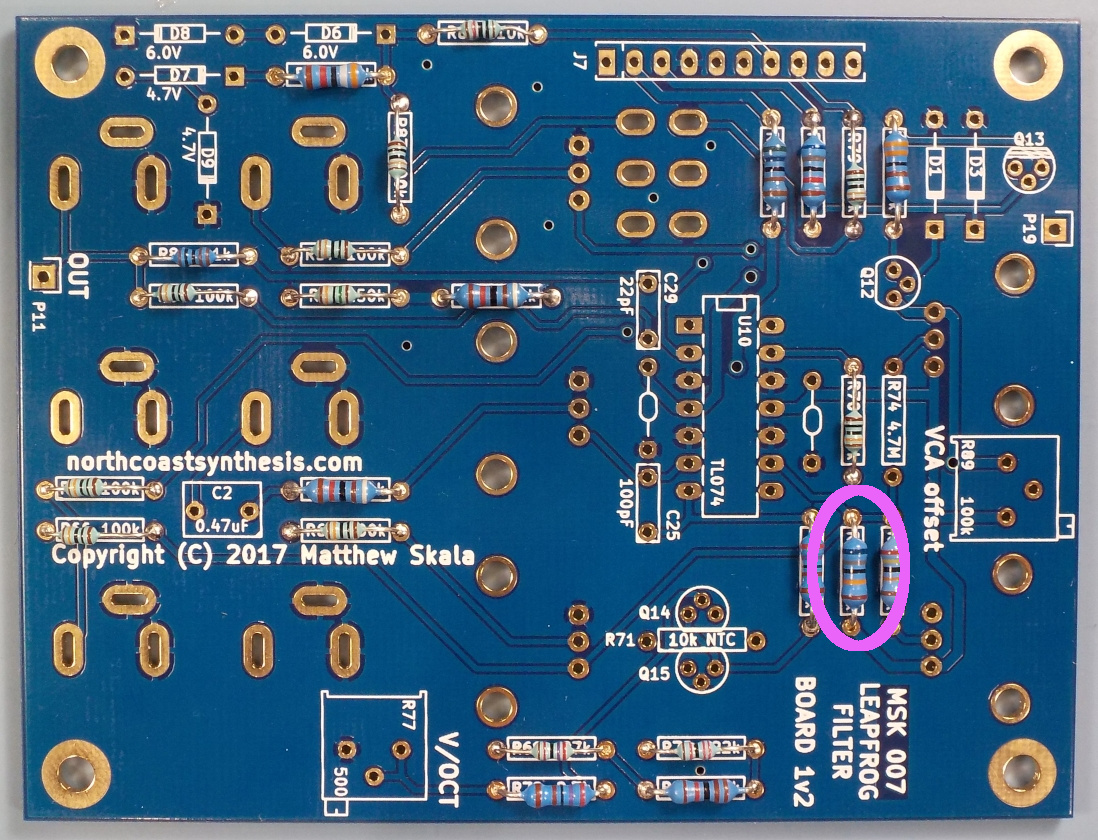
\includegraphics[width=\linewidth]{res-680k1.jpg}

Install the 4.7M$\Omega$ (yellow-violet-black-yellow) resistor R74.
This resistor sets the range of the fine tuning knob to about half an
octave.

\nopagebreak
\noindent\includegraphics[width=\linewidth]{{res-4.7m1}.jpg}

\section{Diodes}

There are six diodes to be mounted on Board~1:  two each of 1N4148 or 1N914
switching diodes; 1N5230B 4.7V Zener diodes; and 1N5223B 6.0V Zener diodes. 
They all look like pretty much identical orange-pink glass beads, and it is
important not to confuse them.  Their bodies will be marked with type
numbers in very small print, and they should be labelled in a kit, but if
you are in any doubt, test them for breakdown voltage.

\pagebreak

To do a breakdown voltage test:  use clip leads or a breadboard to connect
the diode under test in series with a small resistor (anything from
1k$\Omega$ to 10k$\Omega$) reverse biased across a 12V power supply.  That
is, the power supply positive connects to one end of the resistor, the other
end of the resistor connects to the cathode (striped end) of the diode, and
the anode (other end) of the diode connects to the power supply negative. 
Then measure the voltage across the diode.  It should be close to the
specified Zener voltage of 4.7V or 6.0V if you are testing a Zener diode,
and equal to the power supply voltage if you are testing one of the
switching diodes.  From that it should be possible to determine which diodes
are which.  If the measured value is less than 1V, then you most likely have
the diode backwards and are measuring its \emph{forward} voltage, which will
be about the same for all three of these diode types and is not a useful way
to distinguish them.

All these diodes are polarized components and it is important to install
them right way round.  Each diode has a black stripe at one end; that end is
the \emph{cathode}.  The silkscreen markings on the board have a
corresponding stripe and the diodes should be installed with their stripes
matching the markings on the board.  The solder pads for the cathodes are
also square instead of round.

Install the two 1N4148 or 1N914 switching diodes D1 and D3.  These are used
to control the minimum base voltages for the transistors in the VCA section.

\nopagebreak
\noindent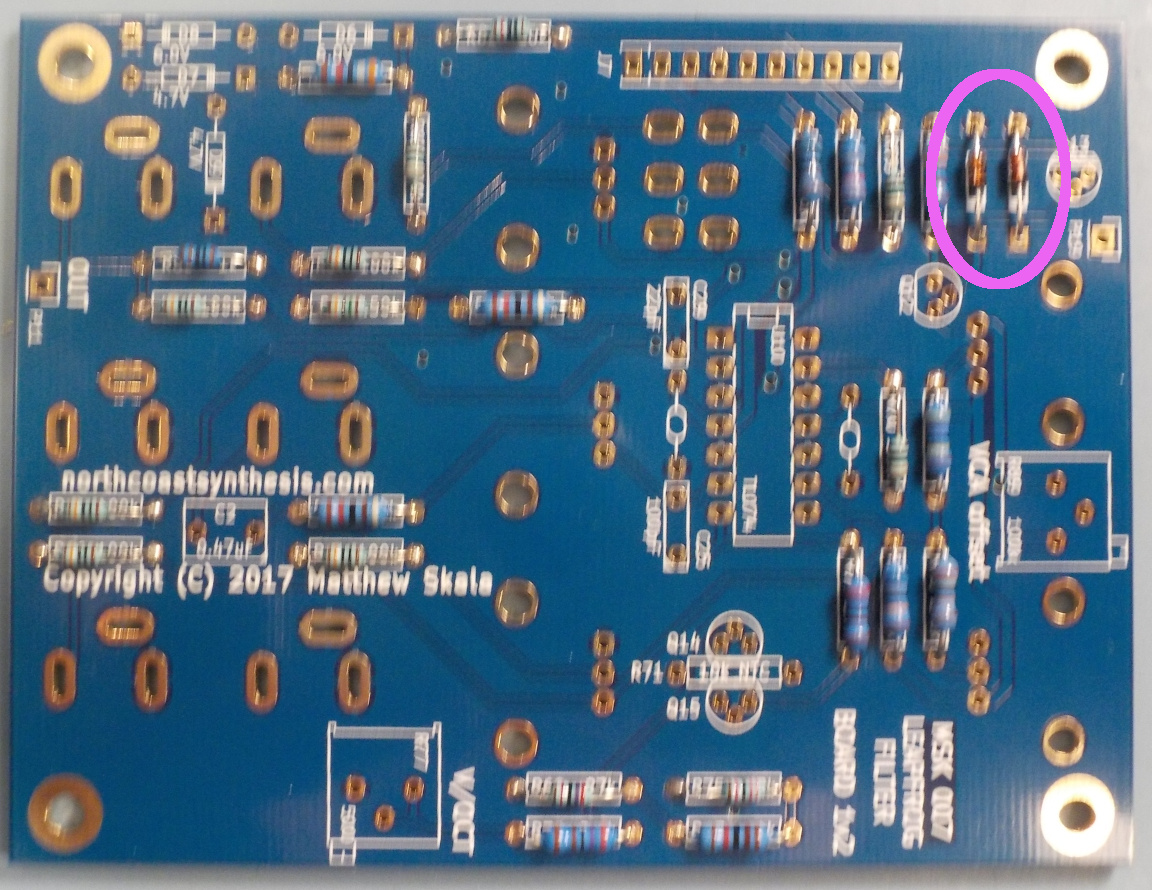
\includegraphics[width=\linewidth]{1n4148.jpg}

\pagebreak

Install the two 1N5230B Zener diodes D7 and D9.  Their breakdown voltage of
4.7V is marked on the silkscreen as an additional guide to where they go. 
These set the lower voltage level for the soft-clipping circuit.

\nopagebreak
\noindent\includegraphics[width=\linewidth]{{zener-4.7v1}.jpg}

Install the two 1N5233B Zener diodes D6 and D8.  Their breakdown voltage of
6.0V is marked on the silkscreen as an additional guide to where they go. 
These set the higher voltage level for the soft-clipping circuit.

\nopagebreak
\noindent\includegraphics[width=\linewidth]{{zener-6.0v1}.jpg}

\section{DIP sockets}

Install the 14-pin DIP socket for the TL074 quad op amp chip U10.  The
amplifiers in this chip are used in the exponential converter and as buffers
between the filter core and the outside world.  See
page~\pageref{pag:dip-sockets} for notes regarding orientation of the
socket, procedure for soldering it flat to the board, and so on.

\noindent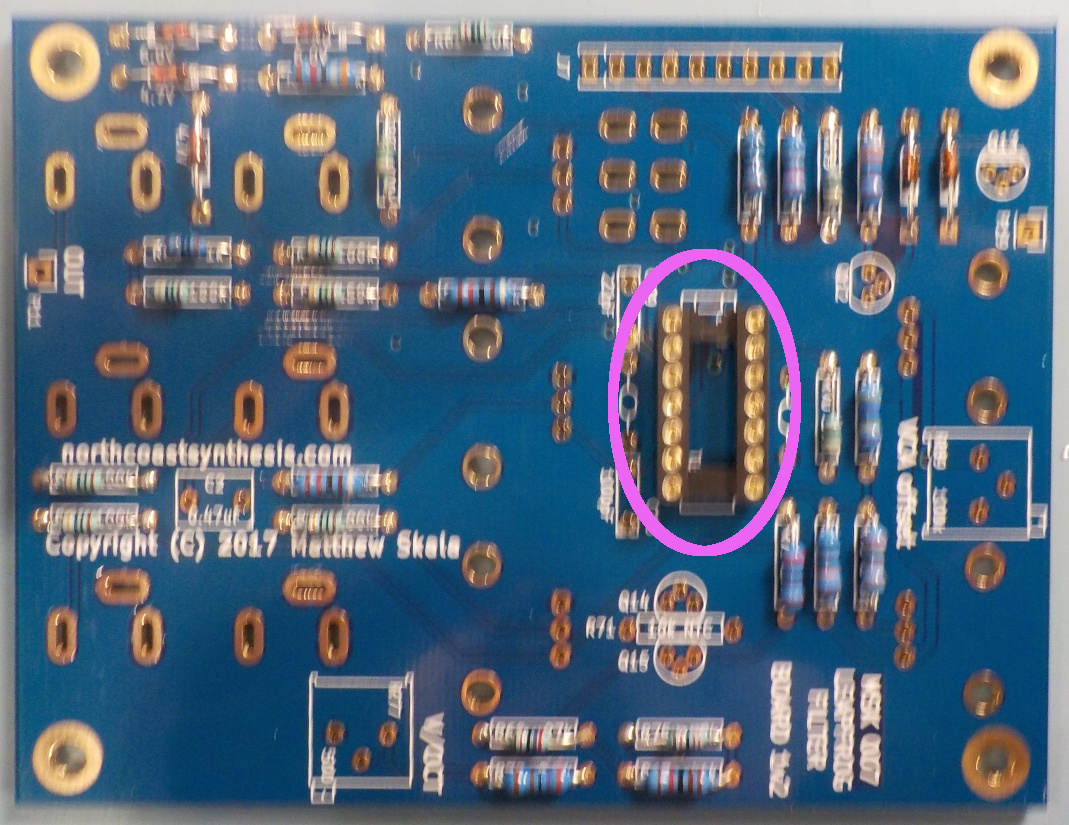
\includegraphics[width=\linewidth]{dip14-1.jpg}

\section{Trimmer potentiometers}

If you have not already set the trimmers to 50\%\ of their full scale value
as described under ``Preliminaries'' above, then do it now.

Trimmers are not exactly polarized, but the three legs of each trimmer serve
different functions and need to be connected to the right holes.  The
physical arrangement of the legs and corresponding holes should make it
impossible to install the trimmers wrong way round.

Install the 500$\Omega$ trimmer R77.  This trimmer sets the scale factor for
the V/octave pitch CV, an adjustment often called ``tracking.''

\nopagebreak
\noindent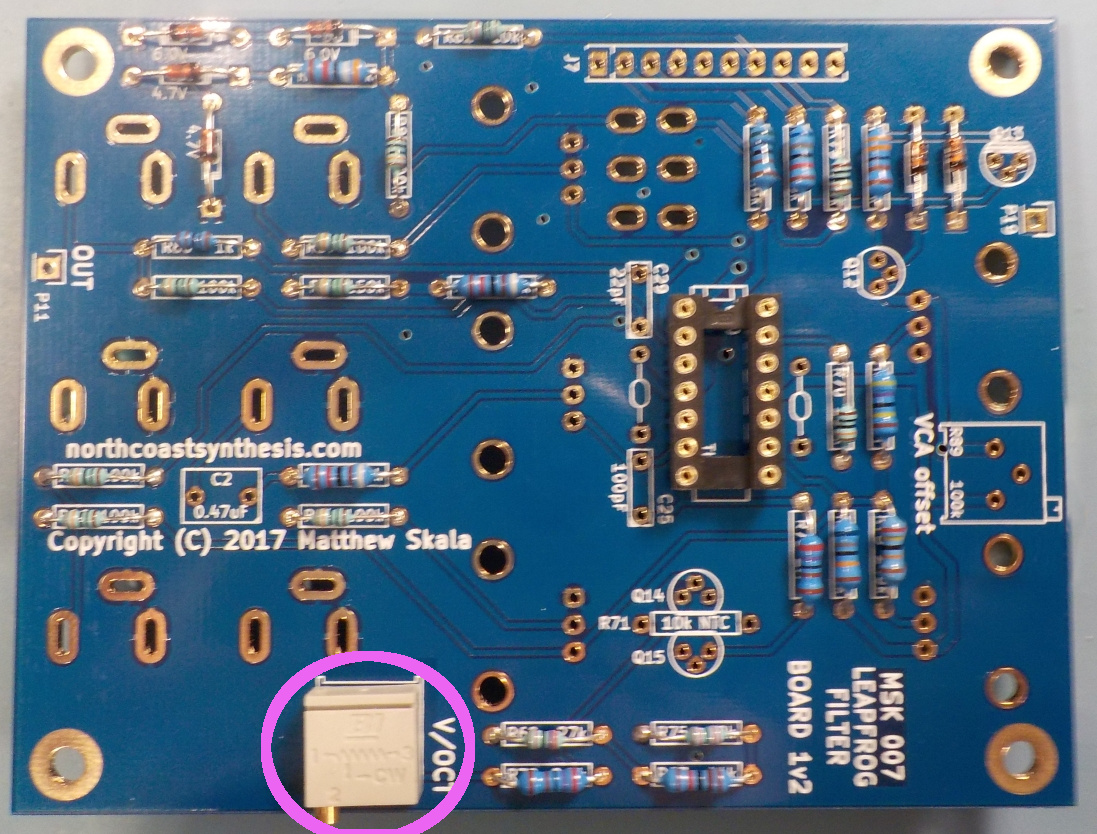
\includegraphics[width=\linewidth]{pot-500w1.jpg}

\pagebreak

Install the 100k$\Omega$ trimmer R89.  This trimmer adjusts the DC offset in
the VCA section.

\nopagebreak
\noindent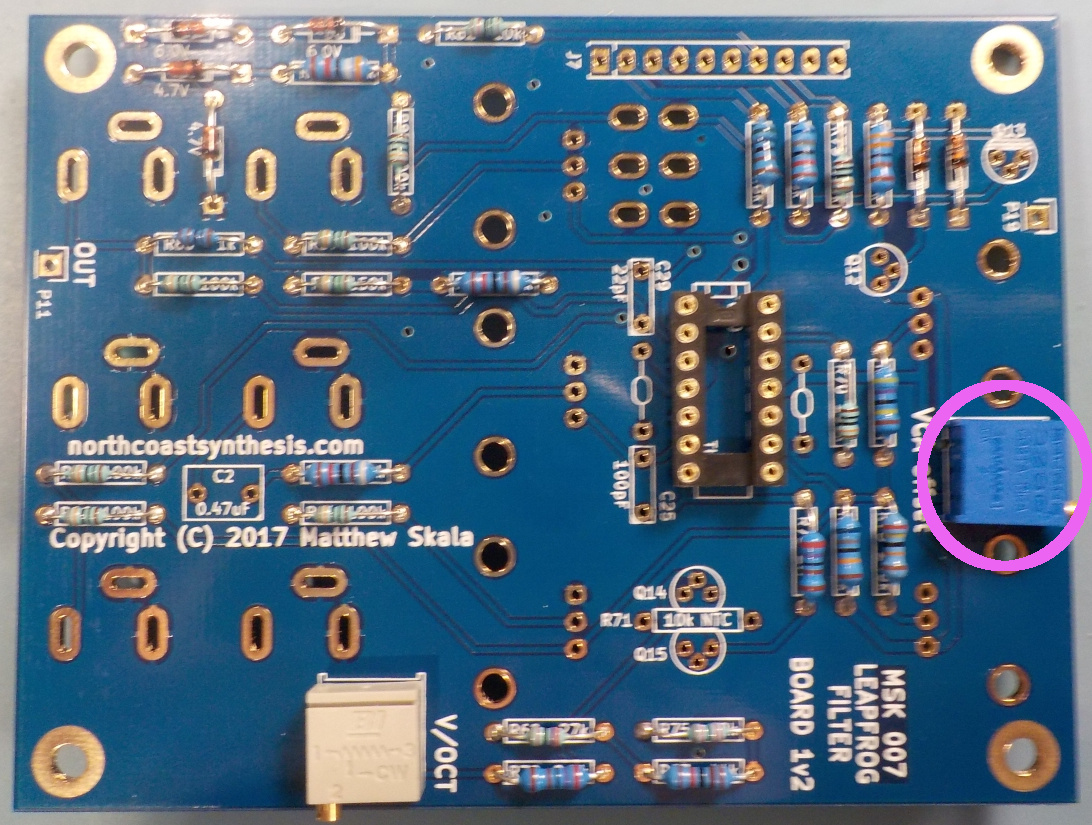
\includegraphics[width=\linewidth]{pot-100k1.jpg}

\section{Capacitors}

Small-valued ceramic capacitors are usually labelled with numbers in a
pattern similar to the resistor colour code:  two digits for the main value,
followed by a third digit that says how many zeroes to append to get the
value in picofarads.  Thus the 22pF capacitor may be labelled ``220'' and
the 100pF capacitor ``101.''  Other markings on the capacitor body may
indicate tolerance, voltage rating, dielectric type, and so on.  The
0.1$\mu$F decoupling capacitors will probably have very abbreviated markings,
but if they are labelled on the three-digit system the code would be ``104''
for 0.1$\mu$F $=$ 100000pF (10 followed by 4 additional zeroes);
and the box-type 0.47$\mu$F film capacitor will likely be marked with its
value in microfarads using $\mu$ instead of the decimal point, thus
``$\mu$47.''  None of the capacitors to be installed on this board are
polarized.

\pagebreak

Install the 22pF ceramic capacitor C29.  This capacitor prevents
high-frequency oscillation of the output driver op amp.

\nopagebreak
\noindent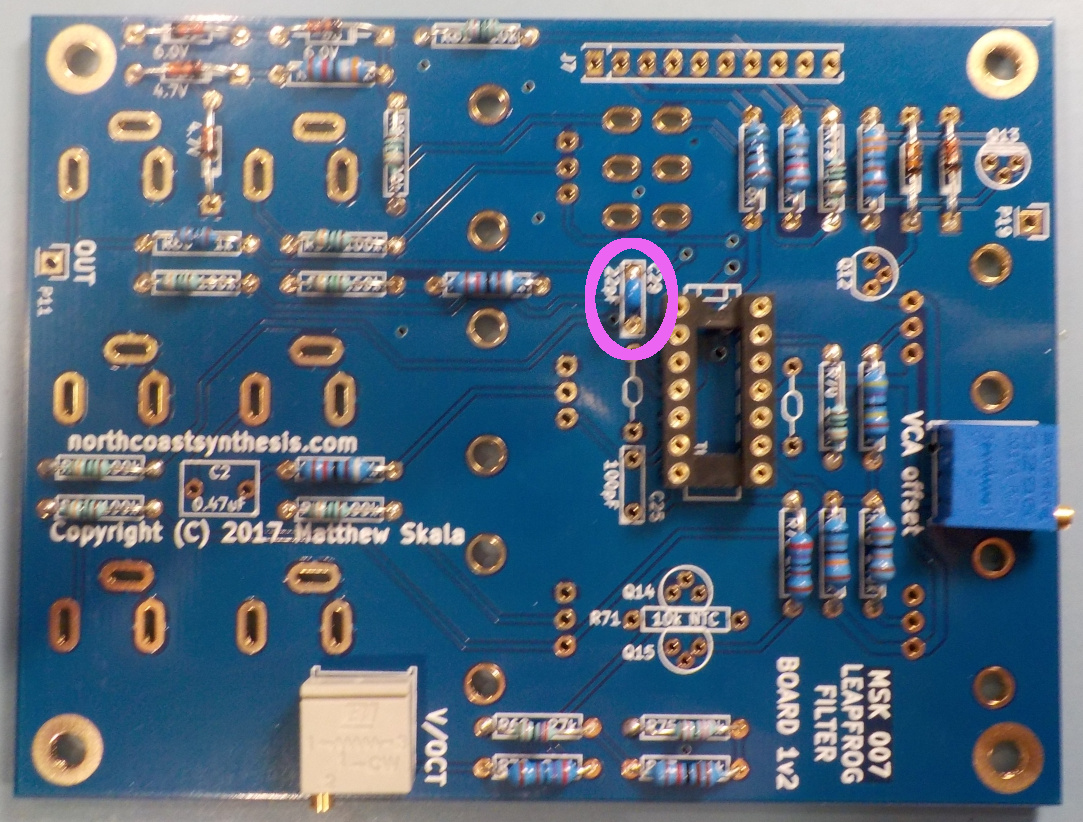
\includegraphics[width=\linewidth]{cap-22p1.jpg}

Install the 100pF ceramic capacitor C25.  This capacitor prevents
high-frequency oscillation of the exponential converter servo op amp.

\nopagebreak
\noindent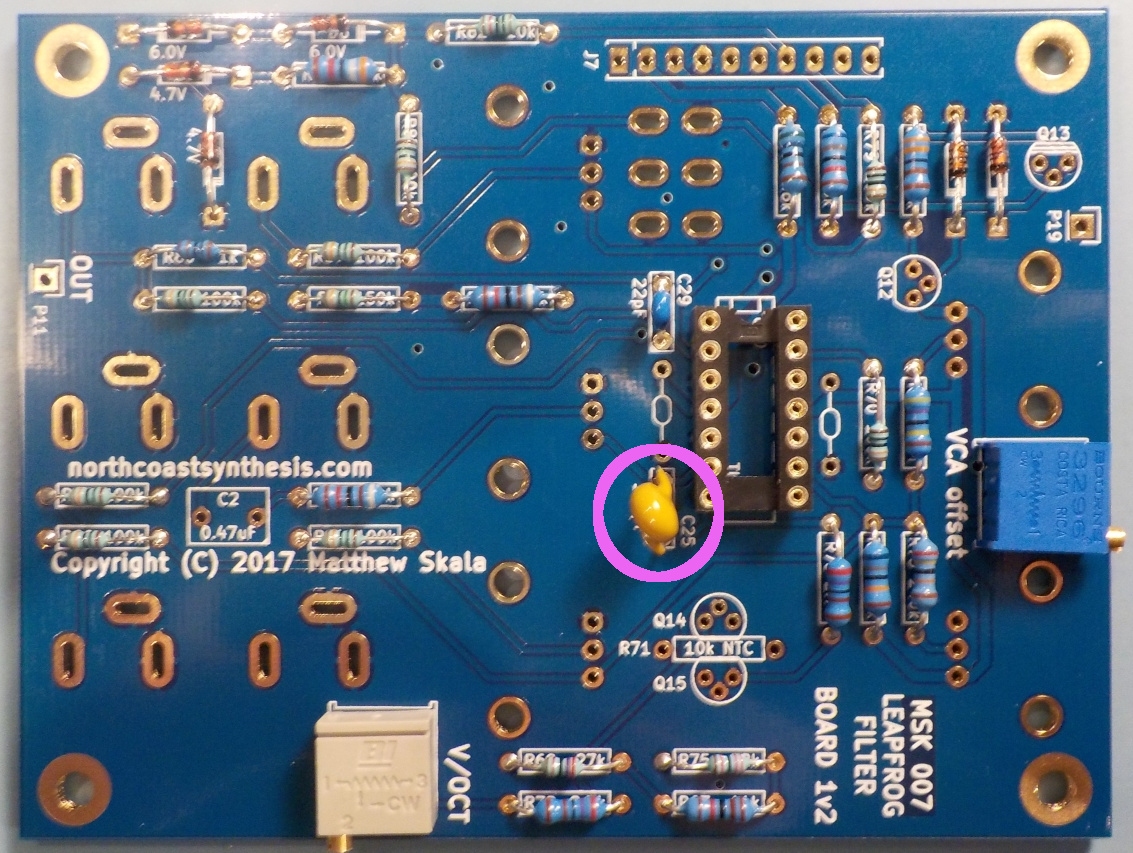
\includegraphics[width=\linewidth]{cap-100p1.jpg}

\pagebreak

Install the two 0.1$\mu$F decoupling capacitors.  As described on
page~\pageref{pag:decoup-symbol}, they are shown on the board silkscreen by
a special symbol without values or reference designators.  They filter the
power supplies for the op amp chip.

\nopagebreak
\noindent\includegraphics[width=\linewidth]{{cap-0.1u1}.jpg}

Install the 0.47$\mu$F film capacitor C2.  This capacitor provides AC
coupling for the linear FM input.

\nopagebreak
\noindent\includegraphics[width=\linewidth]{{cap-0.47u1}.jpg}

\pagebreak

\section{TO-92 semiconductors}

See page~\pageref{pag:to-92} for general instructions regarding TO-92
semiconductors and the board symbols used for them.

Install the PNP transistor Q13, type SS8550D or PN200A.  This transistor
acts as a current source for controlling the VCA section.

\nopagebreak
\noindent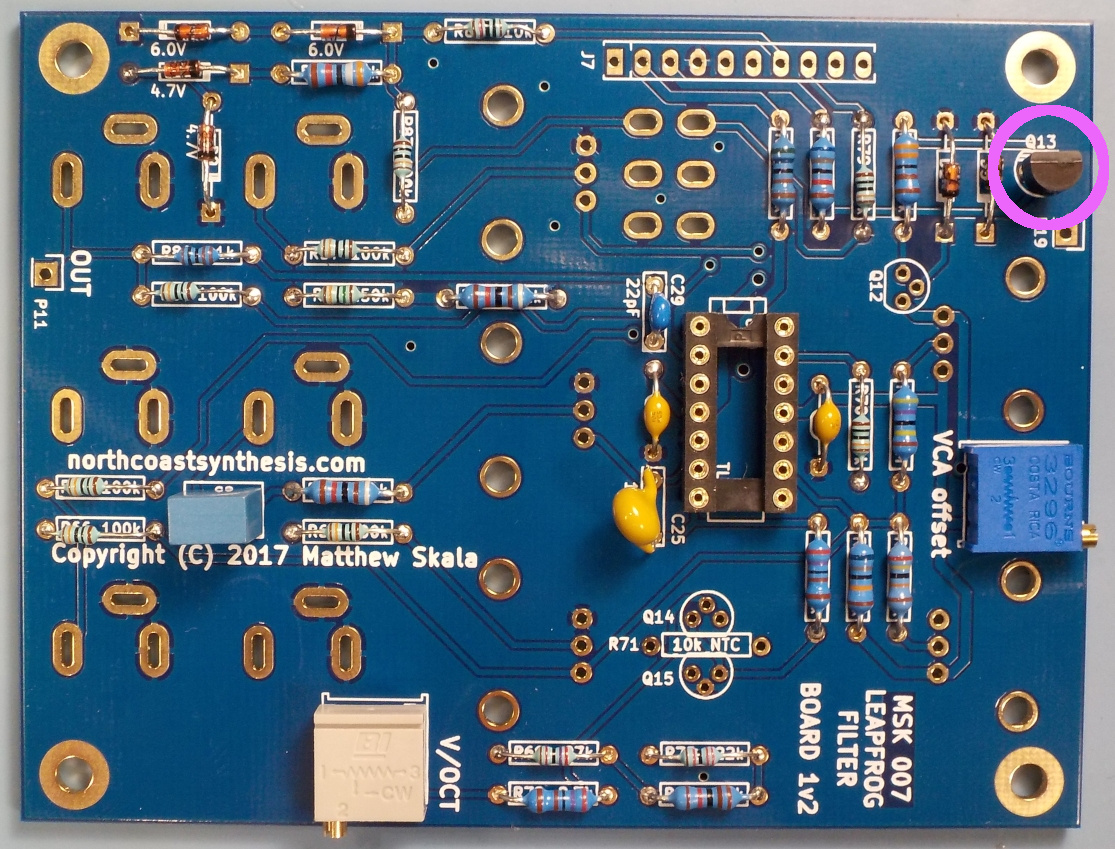
\includegraphics[width=\linewidth]{pn200a-1.jpg}

Install the 2N5088 NPN amplifier transistor Q12.  This transistor acts as an
emitter follower to translate the input control voltage to a current for
Q13.  There are two more 2N5088 transistors to be installed in the next
section.

\nopagebreak
\noindent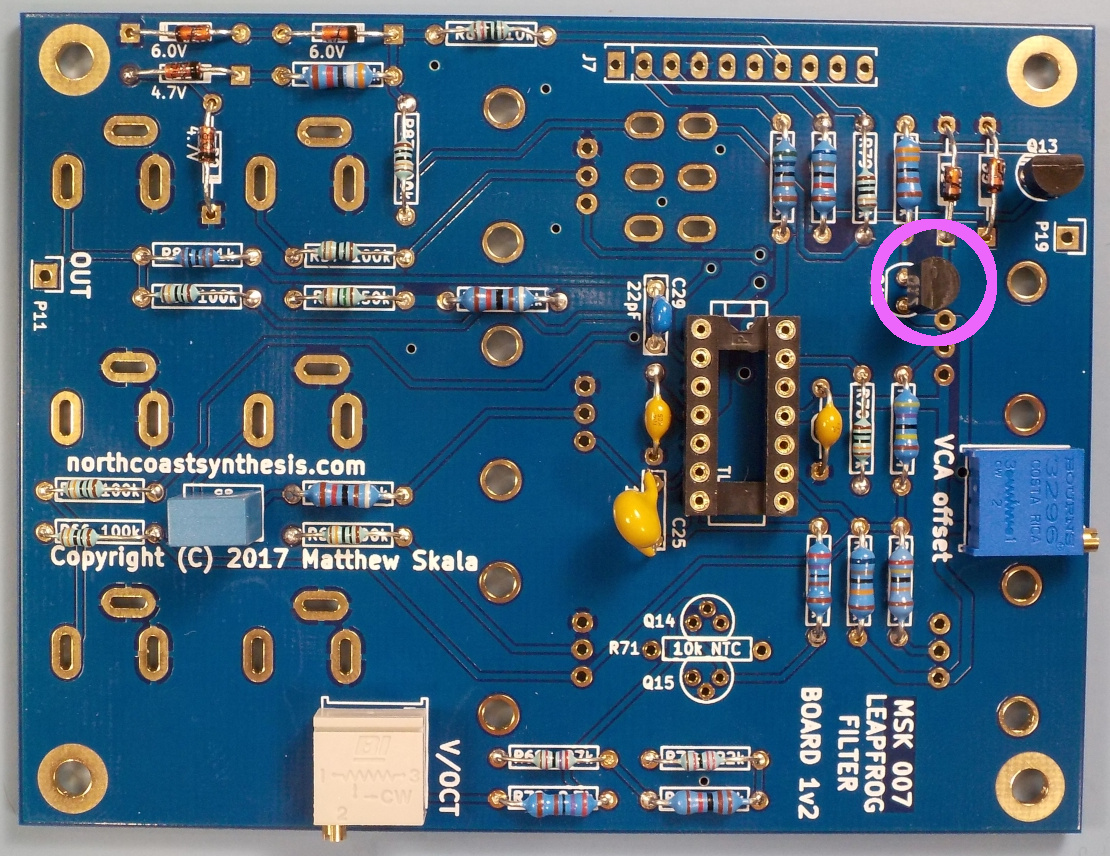
\includegraphics[width=\linewidth]{2n5088-1.jpg}

\section{Exponential converter cluster}

In order to reduce the temperature dependence of the exponential converter
as far as possible, is is important that the two transistors Q14 and Q15,
and the thermistor (temperature-sensitive resistor) R71, should all be kept
at the same temperature.  This is accomplished by mounting them all in
contact with each other and tightening a nylon cable tie around them to keep
them pressed together.  Constructing this cluster of components is a little
tricky and annoying; follow the directions carefully.

Bend the thermistor legs as shown:  one leg straight down, the other down
about 3mm, then to the side, then down again, to fit the R71 footprint. 
Place the thermistor in its footprint, but do not solder it yet.

\nopagebreak
\noindent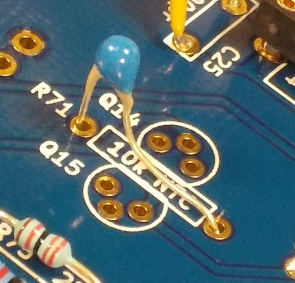
\includegraphics[width=\linewidth]{ntc-bend.jpg}

Insert the two 2N5088 transistors Q14 and Q15 in the board, face to face as
shown.  Do not solder them yet.

\nopagebreak
\noindent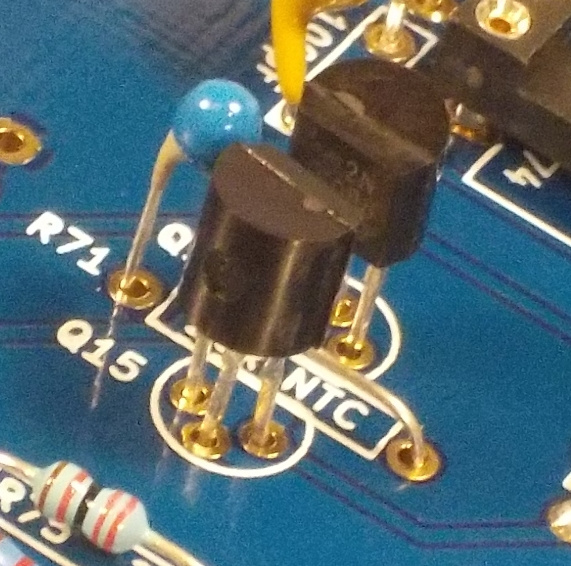
\includegraphics[width=\linewidth]{expo-untied.jpg}

\pagebreak

Put a nylon cable tie around the three components and tighten it far enough
to hold them loosely together.  Concentrate in particular on having the two
transistors meet as cleanly face to face as possible.  Do not overtighten
the cable tie or cut it off yet.  This is probably the hardest step, and
North Coast kits include a spare cable tie for use in case you ruin one.  Be
aware that the components should not stick out any further above the board
than is normal for other TO-92 components; if you seat the transistors too
high up, at the full length of their legs, you may exceed the 11mm of
clearance between this board and Board~2 above it.

Solder the components.  Then tighten the cable tie the rest of the way and
cut off the excess.

\nopagebreak
\noindent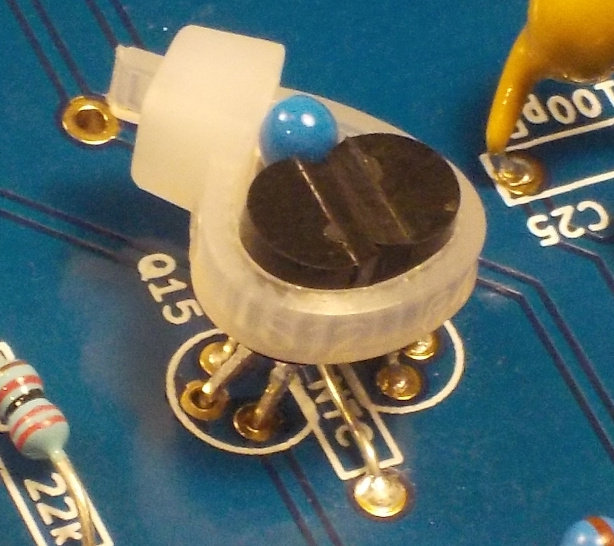
\includegraphics[width=\linewidth]{expo-tied.jpg}

\pagebreak

\section{Board to board connectors}

Screw one 13mm and one 11mm standoff into each of the four mounting holes in
Board~1, as shown.  The shorter (11mm) standoff should be on the top, the
same side as the components already installed, with the male-threaded ends
sticking up.  These standoffs will separate Board~1 from Board~2 in the
final module.  The longer (13mm) standoffs should be on the bottom, with
their male ends passing through the board to mate with the 11mm standoffs.

\nopagebreak
\noindent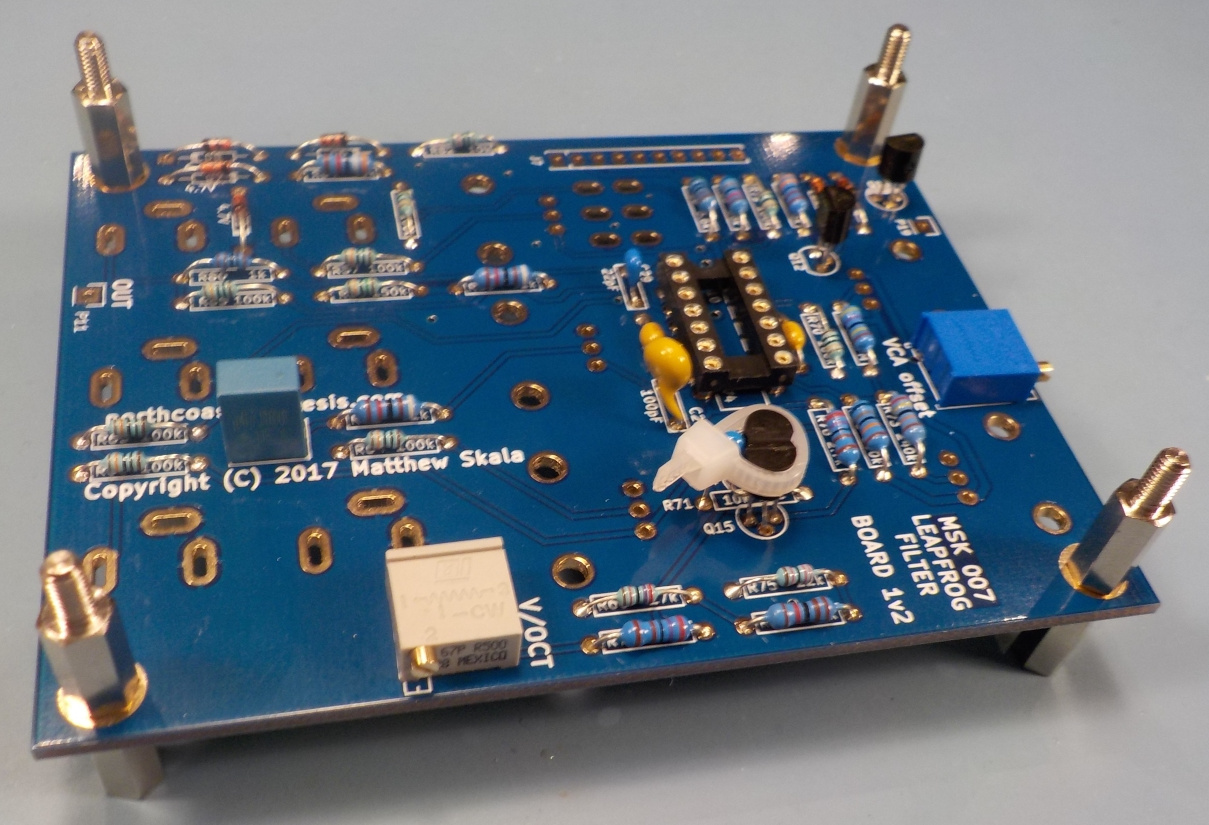
\includegraphics[width=\linewidth]{board12-stack-1.jpg}

Mate the 10$\times$1 header connectors J7 and P26 and place them (do not
solder yet) in the J7 footprint on Board~1 with the legs of the female
connector J7 going through the board.

\nopagebreak
\noindent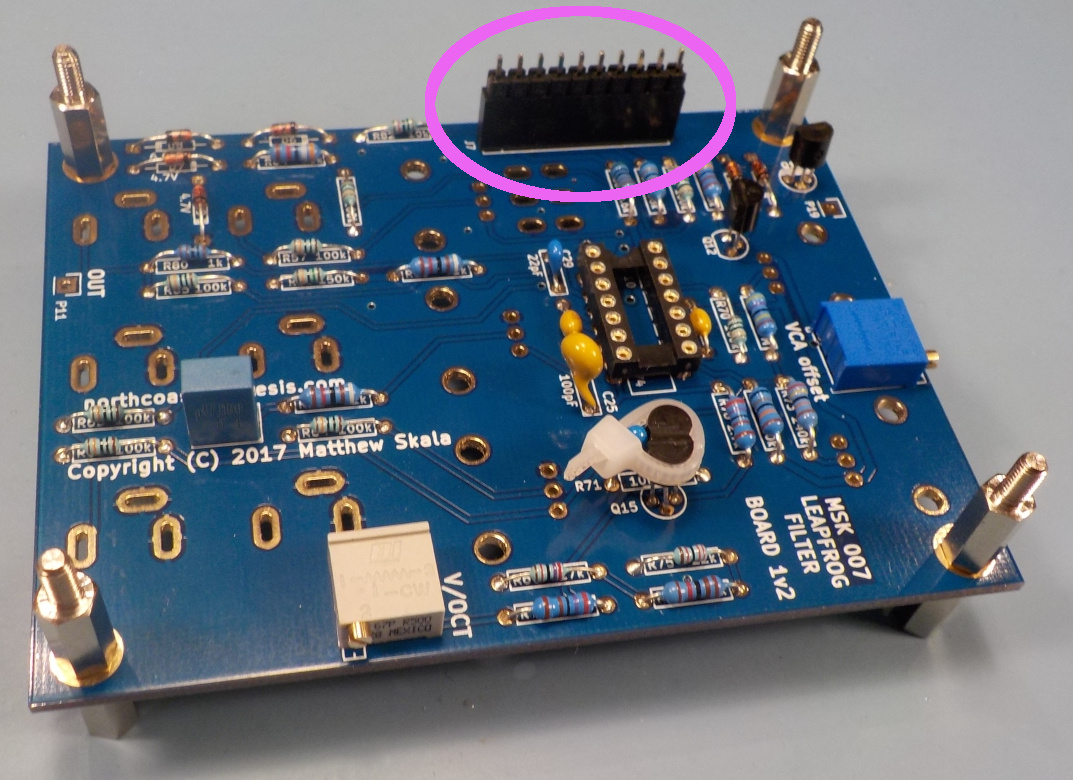
\includegraphics[width=\linewidth]{board12-stack-2.jpg}

\pagebreak

Place your completed Board~2 from the previous chapter on top of the
assembly, component side up with the legs of P26 going through the P26
footprint, and fasten it with the remaining four 11mm standoffs.

\nopagebreak
\noindent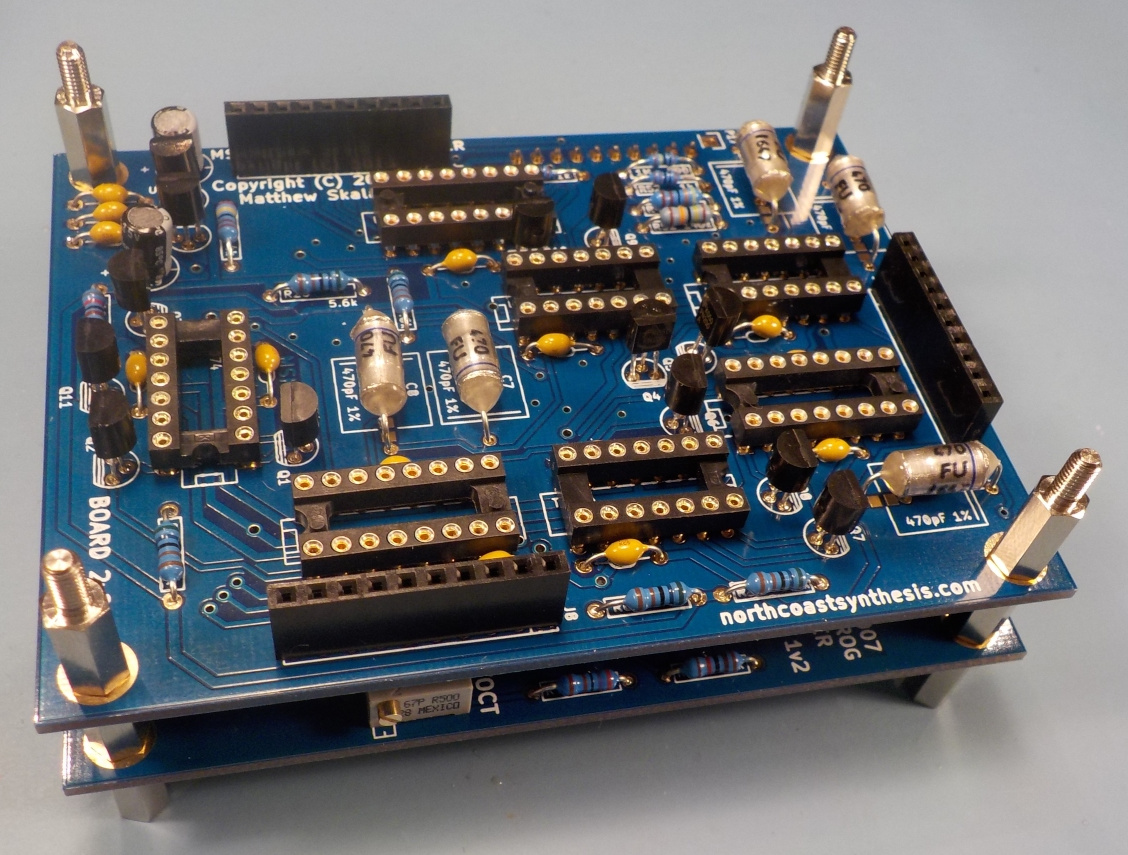
\includegraphics[width=\linewidth]{board12-stack-3.jpg}

Solder J7 and P26 in place on the two boards.  Then remove Board~2 and the
four standoffs holding it in place, but keep the standoffs that go through
the holes in Board~1.

\section{Panel components}

Flip Board~1 over; you will now be installing the components that go between
it and the panel.  The exact details of how the pieces fit together are
important and may not be obvious; see the exploded assembly diagram on
page~\pageref{fig:exploded}, which may clarify things.

The toggle switch SW3 is for switching the VCA section between providing
feedback and controlling the output.  It has a body just a little shorter
than will fit well into the 13mm space between Board~1 and the panel.  This
space is forced to be 13mm to accommodate the potentiometer bodies.  The
switch comes with two nuts and only needs one for fastening on the front of
the panel.  We use the second one as a spacer behind the panel to hold the
switch body far enough back that its legs will go through the holes in the
board.  Remove and save the hardware from the switch bushing, then screw on
one of the nuts all the way down to the bottom of the bushing.

The switch's electrical connections are symmetrical, but it has a slot or
keyway in its bushing, used to hold the special anti-rotation washer in
place.  This keyway must face toward the outer edge of the board in order
for the anti-rotation washer to be able to connect \pagebreak the switch
properly with a matching small hole in the panel.  Place (do not solder yet)
the switch in its footprint on Board~1, with the keyway facing outward.

\nopagebreak
\noindent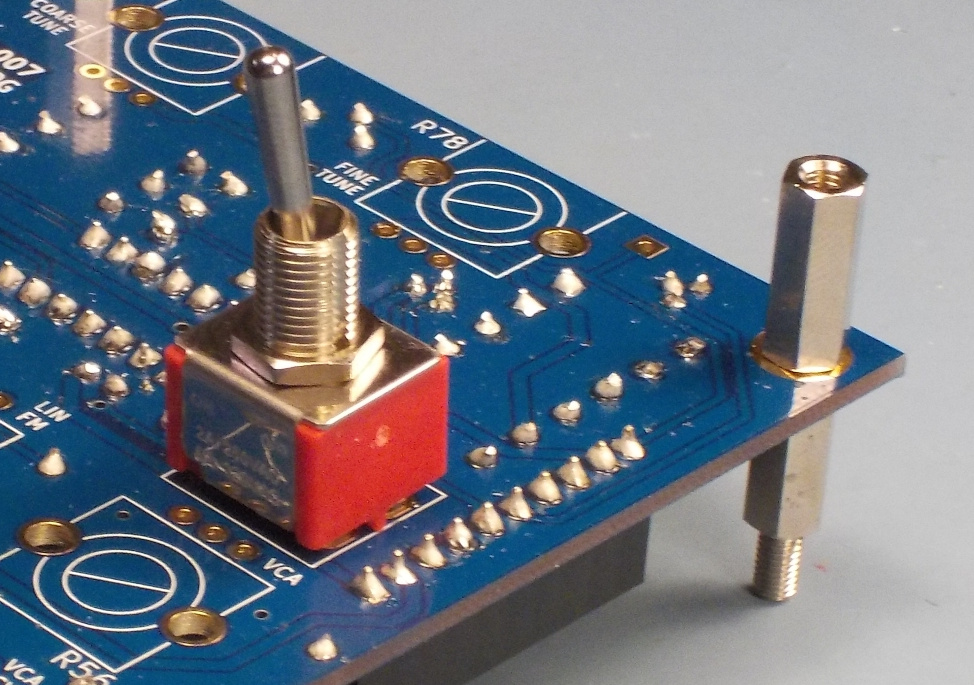
\includegraphics[width=\linewidth]{switch-keyway.jpg}

Place (do not solder yet) the five panel control potentiometers R56, R62,
R69, R78, and R81 in their footprints on the board.  These provide manual
control of the module's functions.  Place (do not solder
yet) the six phone jack sockets J1 through J6 in their footprints.  These
are for patching signals to and from other modules.  All these components
should only be able to fit into the board in one way.

\nopagebreak
\noindent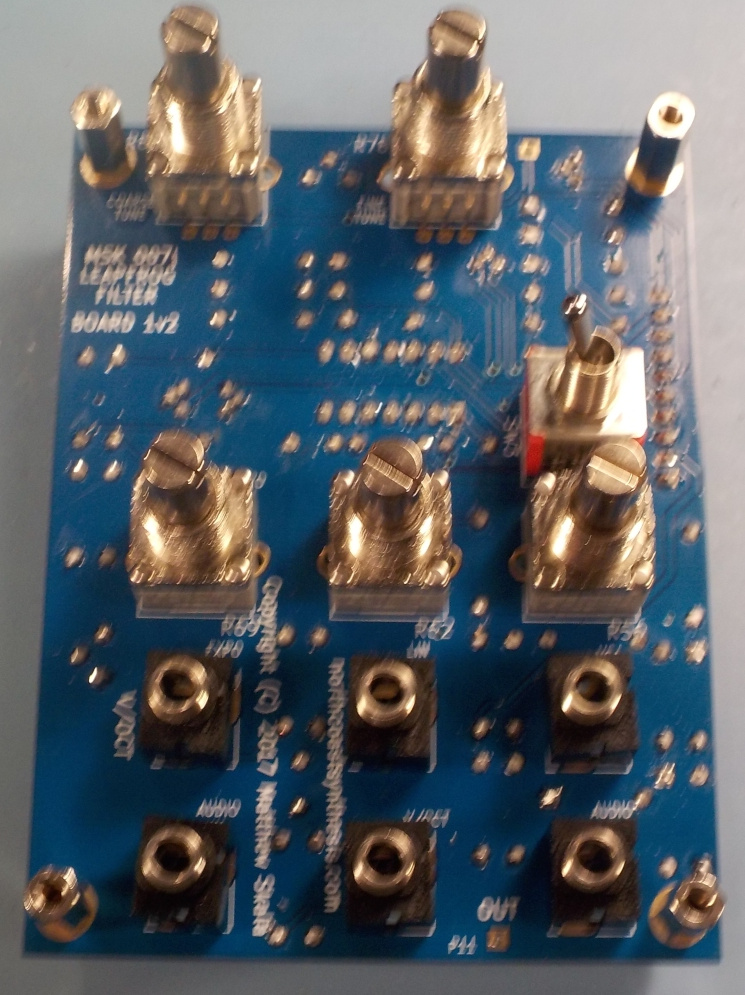
\includegraphics[width=\linewidth]{panel-components.jpg}

Line up the panel on top of the asembly and fasten it in place by driving
the four machine screws through their corresponding holes into the 13mm
standoffs.  Double check that the keyway on the switch bushing is facing the
small hole near the switch which will accept the alignment tab from the
anti-rotation washer.

\noindent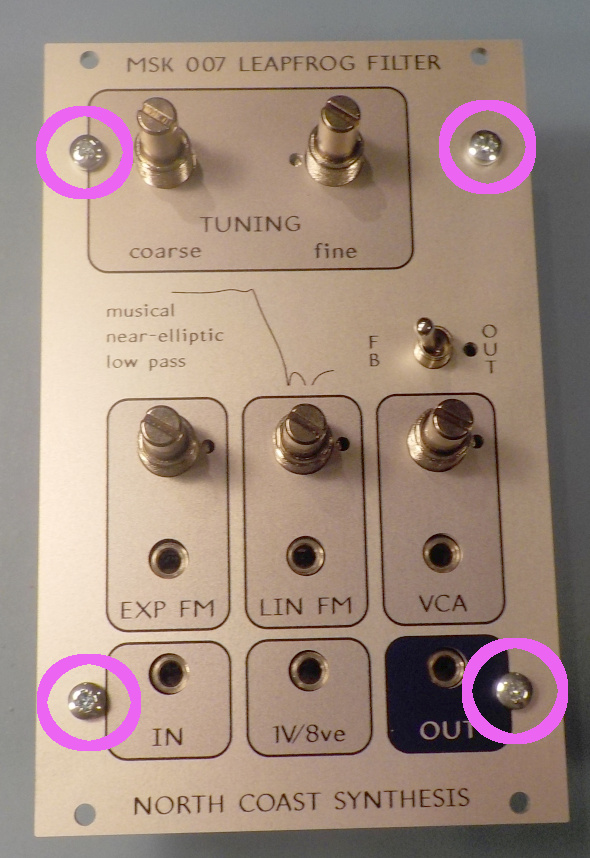
\includegraphics[width=\linewidth]{panel-screws.jpg}

Install all the hardware for the panel components.  In the case of the
switch, the sequence is first (nearest the panel) the anti-rotation washer,
with one of its tabs fitting into the keyway on the bushing and the other
sticking into the small panel hole provided for this purpose; then the
toothed lock-washer (sharper side of the teeth facing up to engage with the
nut, if there's a noticeable difference between the two sides); and finally
the nut.  In the case of the potentiometers, the sequence is first (nearest
the panel) the conical spring washer, high side in the middle and low side
around the outside; then the toothed lock-washer; then the nut.

In the case of the jack sockets, the knurled nuts provided for these will
have screwdriver slots on one side, and those should face the outside with
the smoother side facing the panel.  You may need to tilt the assembly and
jiggle it a bit to get the jack sockets to fall into the right alignment
with their bushings poking through the panel.  On the other side, when
correctly installed their solder legs (and those of the switch) will just
barely pass through the circuit board.

Do not overtighten any of this hardware, and be careful, if you are
using wrenches or pliers, to avoid scratching the panel.  Wrapping the tool
jaws with tape may help.

\nopagebreak
\noindent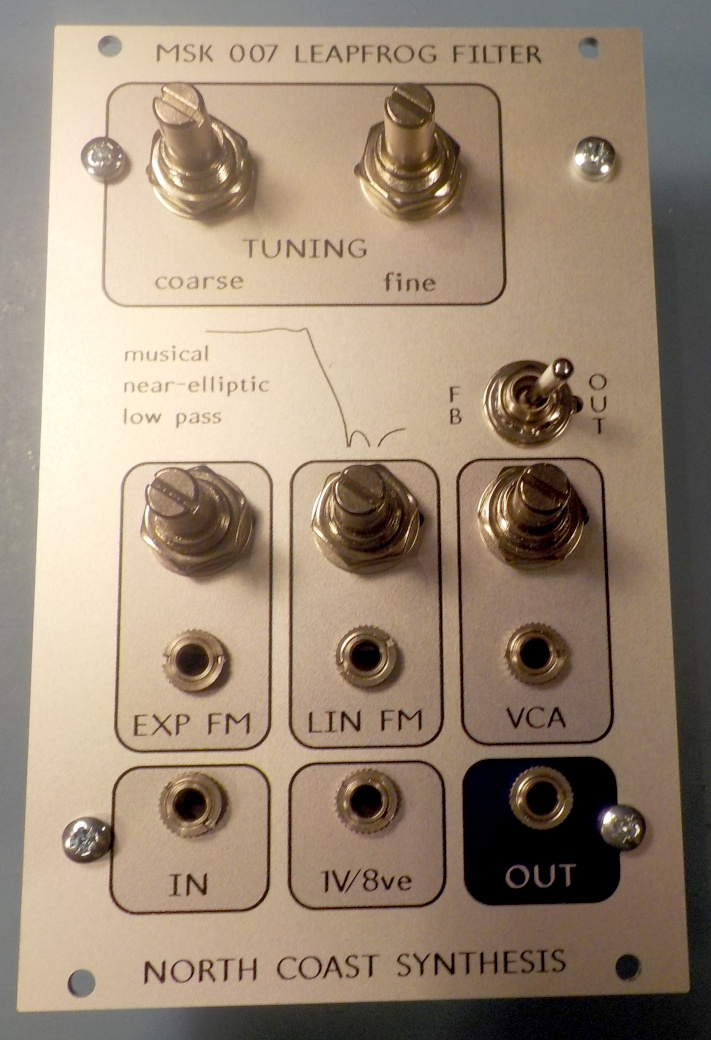
\includegraphics[width=\linewidth]{panel-hardware.jpg}

Solder the panel components.  It can be tricky to do the joints where a
component leg just barely passes through the board, but if you take it slow
and make sure that the PCB hole is filled with solder and the whole joint is
liquid before you remove the heat, then you can be reasonably sure that you
have wetted the leg and made a good electrical connection.  It may help to
use a larger-than-usual soldering iron tip if you have one.

\pagebreak

\section{Final assembly}

Attach the knobs to the potentiometers.  Twist each shaft to its limits in
each direction to ascertain how the slot in the shaft corresponds to where
you want the knob pointer, then slide the knob onto the shaft in the correct
orientation and tighten the setscrew with a small flat screwdriver.  See the
comments at the start of this chapter about knobs, and be sure not to
overtighten the setscrews when attaching them.

Insert a TL047 chip in the U10 socket on Board~1.  Be careful to insert it
right way round: the end with Pin 1 will be marked by an indentation at one
corner or a notch in the end and this end of the chip should be inserted to
match the notch in the socket and on the board silkscreen and the
rectangular Pin 1 solder pad.

Also be careful that all the legs of the chip go into the corresponding
holes in the socket.  These chips, when brand new, usually have their legs
splayed outward a little bit (a measure intended to help them fit snugly
into circuit boards when used without a socket) and you must gently bend the
legs inward in order to fit them in the sockets.  If you apply pressure to a
chip prematurely, without all the legs properly fitting into the holes, it
is easy to have the legs fold up or even break off.

It should not be necessary to remove the panel from Board~1 again.  Attach
Board~2, carefully fitting its header plug into the header socket on Board~1
and the male ends of the standoffs through the corresponding holes in Board~2. 
Screw on the remaining 11mm standoffs to hold it in place.

Insert the remaining four TL074 chips and the three LM13700 chips in their
corresponding sockets.  See the notes above on inserting DIP chips in
general, and pay special attention to the directional markings on the board
silkscreen and the notches in the sockets to make sure you have them
installed in the right directions.

If you have not yet done the ``pre-adjustment'' described in the next
chapter, do it now, before assembling Board~3 with the rest of the module. 
But assuming that is complete, add Board~3 to the assembly, fitting its
three male header connectors into the header sockets on Board~2, and screw
on the four hex nuts to hold it in place.  Be careful with your nutdriver,
pliers, or other tools not to damage other components near the nuts on
Board~3.  If using a nutdriver, socket wrench, or similar, be careful not to
overtighten the nuts:  some tools make it easy to apply more torque than the
threads can sustain.

\pagebreak

There is a rectangular white area on Board~3
reserved for adding a serial number, signature, quality control marking, or
similar.  Use a fine-tipped permanent marker to write whatever you want
there.

Your module is complete.

\nopagebreak
\noindent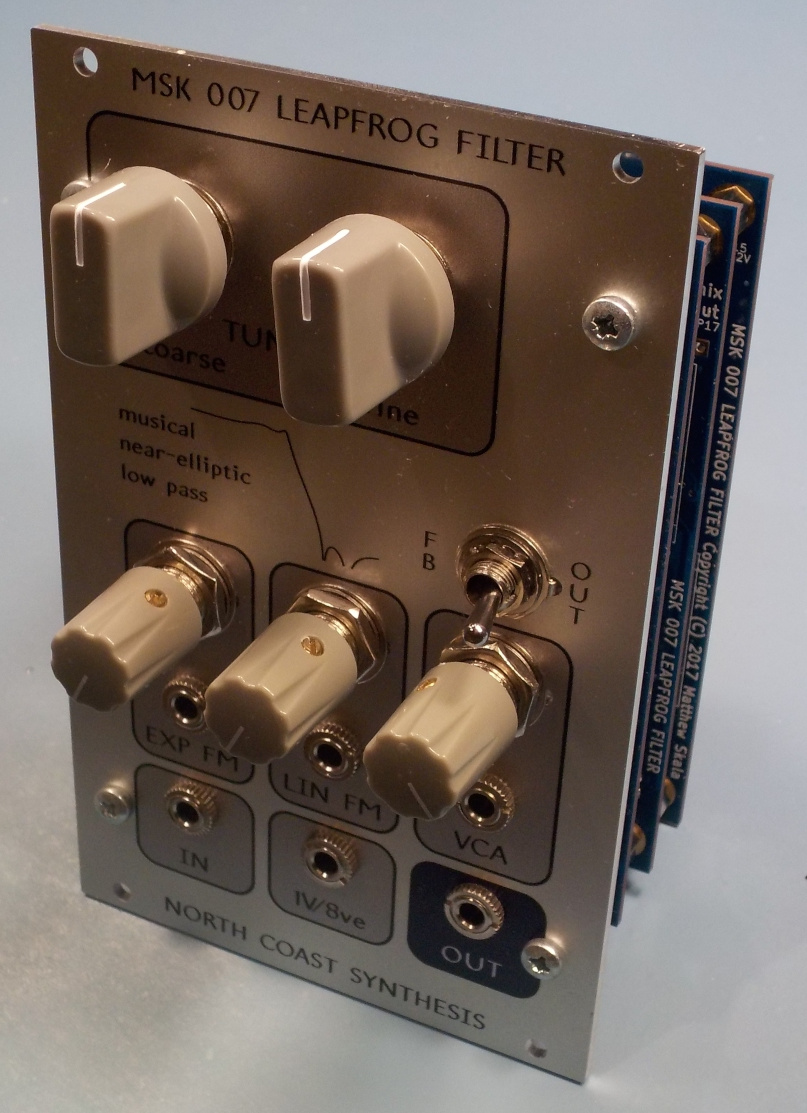
\includegraphics[width=\linewidth]{finished-module.jpg}
